%%%%%%%%%%%%%%%%%%%%%%%%%%%%%%%%%%%%%%%%%%%%%%%%%%%%%%%%%%%%%%%%%%%%%%%%%%%%%%%%
%2345678901234567890123456789012345678901234567890123456789012345678901234567890
%        1         2         3         4         5         6         7         8

\documentclass[letterpaper, 10pt, conference]{ieeeconf}                             
\IEEEoverridecommandlockouts         % Needed if you want to use the \thanks command
                                                     
\overrideIEEEmargins                                                            


\usepackage{times} % assumes new font selection scheme installed
\usepackage{amsmath}
\usepackage{amssymb,longtable,calc}
\usepackage{mathptmx}
\usepackage[T1]{fontenc}                                                        
\usepackage[utf8]{inputenc}                                                     
\usepackage[english]{babel}                                                     
\usepackage{epsfig}                                                             
\usepackage{subfigure}                                                          
\usepackage{textcomp} %<- allows to use \textdegree but may overwrite           
                      %other settings                                           
\usepackage[textwidth=2cm,colorinlistoftodos,disable]{todonotes} %add disable   
                                %to not show the todos                          
\usepackage{tikz}                                                               
\usetikzlibrary{arrows,positioning,fit,shapes,calc}
\usetikzlibrary{matrix}
\usepackage{flushend}                                                           
\usepackage{hyperref}  
\usepackage{amsmath}                                                         
% \usepackage{multirow}   

\usepackage{algorithm}    
\usepackage{algorithmic}

\usepackage{pgfplots} 
\usepackage{pgfplotstable}

\usepackage{cite}

% helper packages to work on the draft
\usepackage[tikz]{bclogo}
\usepackage{lipsum}

\usepackage{standalone}

\pgfplotsset{compat=newest}
\pgfplotsset{ 
  tick label style={font=\footnotesize}, 
  label style={font=\footnotesize}, 
  legend style={font=\footnotesize},
  title style = {font=\small}
}
\pgfplotscreateplotcyclelist{line style}{% 
  solid, mark options = {scale = .75}, every mark/.append style={fill=gray},mark=*\\% 
  densely dashed,mark options = {scale = .75},every mark/.append style={solid,fill=gray},mark=*\\% 
  densely dotted,mark options = {scale = .75},every mark/.append style={solid,fill=gray},mark=*\\% 
  dashed,mark options = {scale = .75},every mark/.append style={solid,fill=gray},mark=*\\% 
  dotted,mark options = {scale = .75},every mark/.append style={solid,fill=gray},mark=*\\% 
}
\pgfplotscreateplotcyclelist{bar style}{% 
  solid, fill=black!60!white\\%
  solid, fill=black!45!white\\%
  solid, fill=black!35!white\\%
  solid, fill=black!25!white\\%
}


\usepackage{xspace}
\makeatletter                                                                   
\DeclareTextCommandDefault{\textregisteredalt}{\footnotesize\textcircled{%      
      \check@mathfonts\fontsize\sf@size\z@\math@fontsfalse\selectfont R}}       
\DeclareRobustCommand\onedot{\futurelet\@let@token\@onedot}                     
\def\@onedot{\ifx\@let@token.\else.\null\fi\xspace}                             
\def\eg{e.g\onedot}                                                             
\def\ie{i.e\onedot}                                                             
\def\vgl{see }                                                                  
\def\Fig{Fig\onedot }                                                           
\def\Tab{Tab\onedot }                                                           
\def\Eq{Eq\onedot }
\def\Sec{Sec\onedot}                                                            
\def\etc{etc\onedot}                                                            
\def\etal{\textsl{et al}\onedot}                                                
\def\argmin{\mathop{\rm arg\,min}}                                              
\makeatother
                                                                    
\definecolor{lightGray}{rgb}{0.0,0.0,0.0}
                                                                                
\title{\LARGE \bf Feature Descriptors for Tracking by Detection: a Benchmark}                                                                               
                                                                                
                                                                                
\author{Alessandro Pieropan ~~~~ Mårten Bj{\"o}rkman  ~~~~ Niklas Bergstr{\"o}m ~~~~  Masatoshi Ishikawa ~~~~ Danica Kragic%
\thanks{The GPU used for this research was donated by the NVIDIA Corporation.}
\thanks{MB and DN are with CVAP/CAS, KTH, Stockholm, Sweden, {\tt celle,dani@kth.se}. AP, NB and MI are with the University of Tokyo, Japan, {\tt }.}}

\begin{document}                                                                
                                                                                
\maketitle                                                                      
\thispagestyle{empty}                                                           
\pagestyle{empty}



%%%%%%%%%%%%%%%%%%%%%%%%%%%%%% ABSTRACT %%%%%%%%%%%%%%%%%%%%%%%%%%%%%%%%%%%%%
\begin{abstract}

Humans are able to merge information from multiple perceptional modalities and formulate a 
coherent representation of the world. Our thesis is that robots need to do the same in order to operate robustly and autonomously in an unstructured environment. 
It has also been shown in several fields that multiple sources of information can complement each other,  overcoming the limitations of a single perceptual modality.
Hence, in this paper we introduce a data set of actions that includes both 
visual data (RGB-D video and 6DOF object pose estimation) and 
acoustic data. We also propose a method for recognizing and segmenting actions from 
continuous audio-visual data. The proposed method is employed for extensive evaluation
of the descriptive power of the two modalities, and we discuss how they 
can be used jointly to infer a coherent interpretation of the recorded action.

\end{abstract}

%%%%%%%%%%%%%%%%%%%%%%%%%%%%%% INTRODUCTION %%%%%%%%%%%%%%%%%%%%%%%%%%%%%%%%%%%
% \begin{}
\section{INTRODUCTION}
\label{sec:introduction}


There has been tremendous effort in the robotics community to develop robots able to operate autonomously in unstructured environments. Robots should be able to perceive the world correctly, detect objects, observe and interact with humans, perform activities and understand if the desired outcome has been achieved \cite{montesano08}.

Much effort has been spent on development of methods for visual perception and modeling of scenes. Many successful solutions have been proposed, considering various visual aspects such as object appearance, motion, human pose and affordances. %A challenge that these perception algorithms have in common is to integrate different kinds of information to formulate a consistent interpretation of the data. This approach strictly relates to the binding problem \cite{Treisman96} known in neuroscience. 
Nevertheless, the use of visual features has some limitations. Firstly, an action has to be performed within the field of view of the observer in order to be perceived. Secondly, object detection and tracking are very sensitive to occlusions while performing activities. Finally, there are meaningful states induced by an action that are hard to detect just relying on visual perception, it is, e.g., very difficult to detect if a person has turned on an oven.

One approach to tackle these limitation is to use additional sources of information, e.g., audio. While this field was in the past more focused on solving problems such as source localization and noise filtering, lately, the focus is more on exploiting sound to extract semantic knowledge and perform scene understanding \cite{Lyon10}. In many contexts, such information is very descriptive and can be helpful to understand a scene. Potentially it could compensate the limitations of visual perception (Fig.~\ref{fig:intro}). However, an important question arises: how can different modalities contribute to formulate a coherent interpretation of the world an agent is observing, in a manner similar to how humans process and integrate multiple modalities  \cite{Zmigrod13}?  Multimodality has up to now received relatively little focus in the robotics community, with some exceptions, e.g.,  \cite{TeoYDFA12}, and the task of audio-visual action recognition has not, to our knowledge, been addressed in robotics.



%\begin{figure}[t]
%	\vspace{2mm}
%\centerline{%
%	\subfigure[RGB-D video]{\includegraphics[width=0.48\linewidth]{images/intro/intro_rgb.png}}
%	%\includegraphics[width=0.48\linewidth]{images/intro/intro_disp.png}\label{fig:intro_rgbd}}}
%	%\centerline{%
%	\subfigure[Audio]{\includegraphics[width=0.48\linewidth]{images/intro/audio_intro.png}\label{fig:intro_audio}}}
%	%subfigure[Objects pose]{\includegraphics[width=0.48\linewidth]{images/intro/intro_track.png}\label{fig:intro_objects}}}
%\caption{An RGB-D video modality and an audio modality give complementary information about an observed human action. This is a motivation of why to use a recognition method that takes both modalities into account.}
%\vspace{-3mm}
%\label{fig:intro}
%\end{figure}

The main contribution of this paper is a {\em method for audio-visual recognition of human manipulation actions}. The visual features (Section \ref{sec:extractVideo}) are the relative 3D orientations and positions of objects involved in the activity, while the audio is represented in terms of MFCC features \cite{Hasan04} (Section \ref{sec:extractAudio}). Objects are tracked in 3D from an RGB-D video stream using the method in \cite{KarlTracker} (Section \ref{sec:tracker}). The audio and video cues are fused in an HMM framework (Section \ref{sec:model}). 

An additional contribution of the paper is an {\em RGB-D-audio dataset of humans involved in the activity of making milk and cereals} (Section \ref{sec:dataset}).  This composite activity consists of many sub-actions such as opening and closing boxes and bottles, and pouring milk and cereal. The recognition method described above was evaluated on this dataset (Section \ref{sec:experiments}). The dataset is annotated with manually extracted segmentation points between sub-actions, and 3D positions and orientations of objects, obtained as described above. It also features 3D models of all objects involved. We release source code for administration of and access to the dataset.


%% %%%%%%%%%%%%%%%%%%%%%%%%%%% RELATED WORK %%%%%%%%%%%%%%%%%%%%%%%%%%%%%%%% 
%\section{Related Work}
\label{sec:relatedwork}


Modeling and recognition of human activity from visual perception is an important problem tackled by the computer vision community, with applications in a wide variety of domains including health monitoring, visual surveillance, video search, human computer interaction and robot learning from demonstration. It has been shown \cite{desai10,gupta09a,kjellstrombook11,kjellstromCVIU11,laptev08,moore99,peursum05,veloso05,wu07} that it is advantageous to represent human activity both in terms of human motion and the objects involved in the activity. Several approaches are widely used to tackle this problem. \cite{Sapp10,AslamBB10a} estimate the human body pose  to recognize human activities. \cite{Bobick01} estimates human motion trajectories to infer activities. \cite{Laptev03} recognizes actions in videos by extracting low level spatio-temporal feature descriptors. 

However in the context of robot learning from demonstration it is meaningful to focus the attention on descriptive features that encodes how objects are being used by a human \cite{billard08},\cite{lang-toussaint10} to achieve a task. It is then possible that the robot can imitate the human and operate autonomously to accomplish given tasks. This has been confirmed in recent works  \cite{gall11,grabner11,rivlin95,stark-bowyer96,sutton-stark08,turek10} and it is supported by Gibson's affordance theory \cite{gibson79}, which states that humans and animals recognize objects in terms of function, in a task oriented manner.

\cite{aksoy10,luo11} present a global representation of activities in terms of spatial relations between objects. The recognition of activities is determined on a set of pre-defined symbols which describe the relationships between segmented coherent regions. In our previous work we have show that is also possible to describe object functionality in terms of how they are being handled by a human \cite{pieropan13}.
Moreover, \cite{grabner11} simulates humans performing activities using objects and cluster them into functional classes. In \cite{gupta11,moldovan12,gall11}, real humans are instead observed in interaction with a scene.

Visual perception supply part of the information to interpret the world. Much can be done from the auditory perspective. In \cite{SalviEtAlAffSpeech2012} learning object affordances was extended to auditory perception. However, the acoustic information was in the form of linguistic descriptions of the scene. In this work, on the contrary, we use the sound generated directly by the interaction between objects as a result of human actions. This is similar to what has been done in \cite{Stork12}. However what we propose here is to go one step further, we want to evaluate different sources of information in order to find the limitations and see how they can be jointly used to overcome such limitations. This is in the spirit with a similar work \cite{TeoYDFA12} where language has been exploited to perform action recognition. in order and tackle the same problem but at a higher level using information or features coming from different perceptual input. 

Most of the cited works tackles what is known in neuroscience as the binding problem \cite{Treisman96}, our brain formulate a coherent interpretation of the world from complex input merging multiple sources of information. Such a skill should be taken into account to develop autonomous robots.














%% %%%%%%%%%%%%%%%%%%%%%%%%%%% DATASET AND EVALUATION DESCRIPTION %%%%%%%%%%%%%%%%%%%%%%%%%%%%%%%%
%\input{dataset}

%% %%%%%%%%%%%%%%%%%%%%%%%%%%% BENCHMARK %%%%%%%%%%%%%%%%%%%%%%%%%%%%%%%%
\section{Benchmark}

The purpose of the experiments conducted are three-fold. First we want to measure the descriptiveness of the feature descriptors for matching purposes, this is crucial for the recovery of a tracker upon object loss. Second we measure the tracking accuracy by integrating each feature descriptor in our 2D tracker and compute the overlap measure using the estimated object position. Third we profile each separate step required in tracking by detection (key-point detection, descriptor computation and feature match) in order to evaluate the performance of the feature descriptors for real-time frameworks.

\subsection{Dataset}

\begin{figure*}[t]
	\vspace{2mm}
\centerline{%
	\subfigure{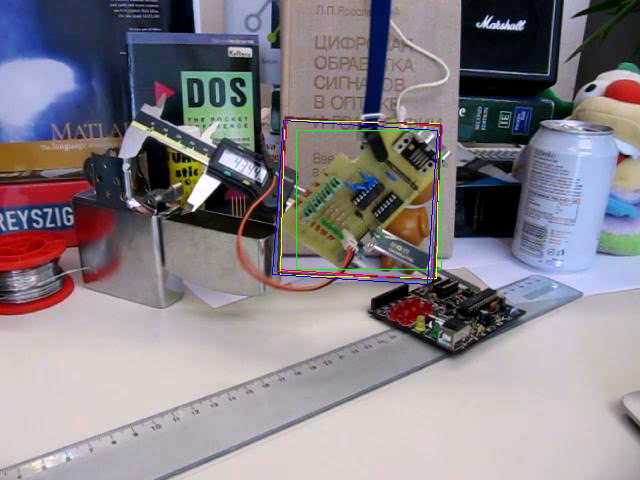
\includegraphics[width=0.19\linewidth]{imgs/dataset/d1.png}}
	\subfigure{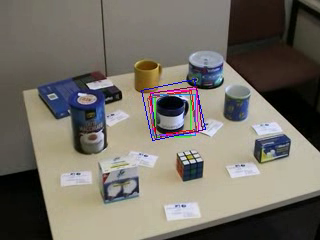
\includegraphics[width=0.19\linewidth]{imgs/dataset/d2.png}}
	\subfigure{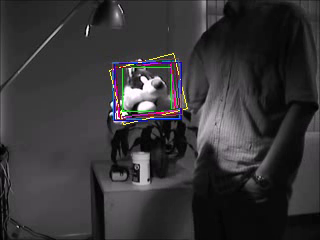
\includegraphics[width=0.19\linewidth]{imgs/dataset/d3.png}}
	\subfigure{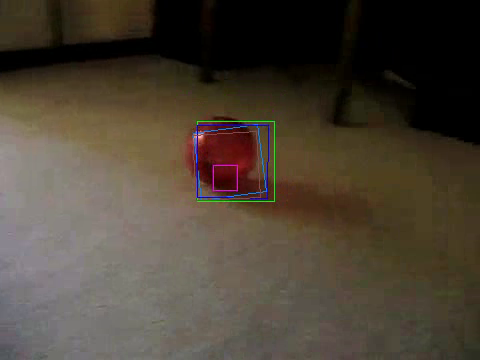
\includegraphics[width=0.19\linewidth]{imgs/dataset/d4.png}}
	\subfigure{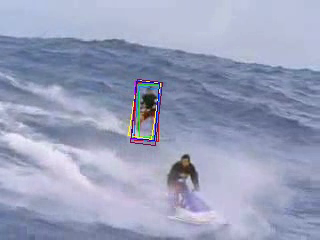
\includegraphics[width=0.19\linewidth]{imgs/dataset/d5.png}}}
	\vspace{-2mm}
\centerline{%
	\subfigure{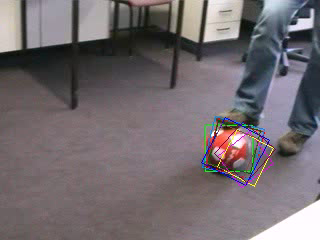
\includegraphics[width=0.19\linewidth]{imgs/dataset/d6.png}}
	\subfigure{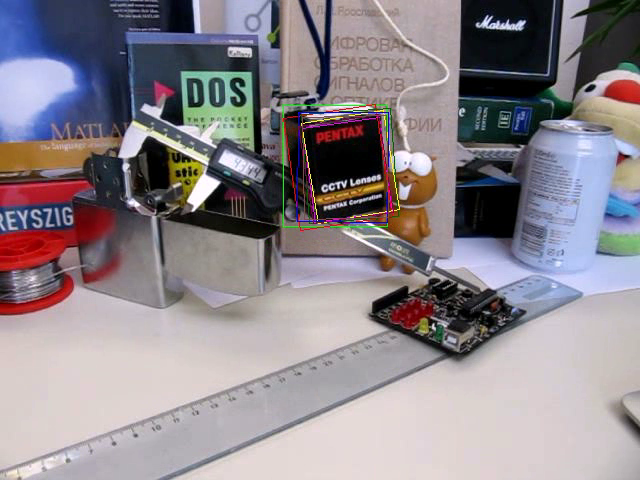
\includegraphics[width=0.19\linewidth]{imgs/dataset/d7.png}}
	\subfigure{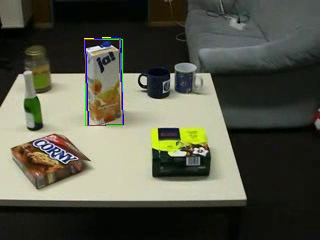
\includegraphics[width=0.19\linewidth]{imgs/dataset/d8.png}}
	\subfigure{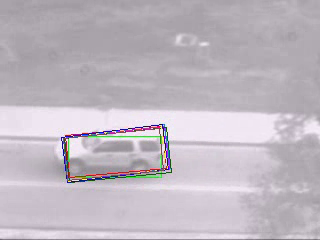
\includegraphics[width=0.19\linewidth]{imgs/dataset/d9.png}}
	\subfigure{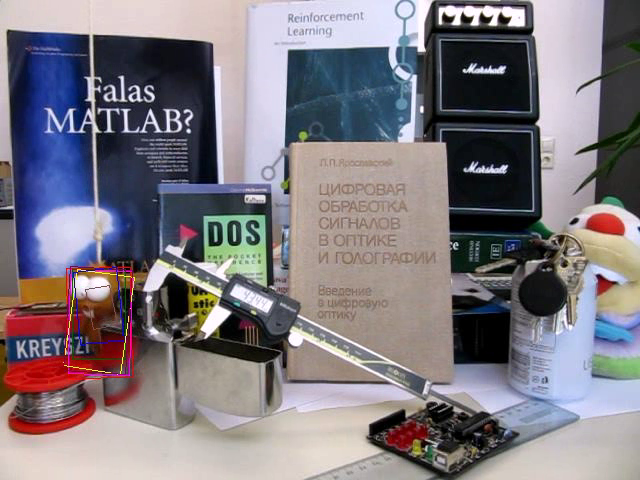
\includegraphics[width=0.19\linewidth]{imgs/dataset/d10.png}}}
\caption{The sequences of the dataset includes both indoor and outdoor scenarios with different light conditions.}
\vspace{-3mm}
\label{fig:data_example}
\end{figure*}


There are many publicly available datasets designed for tracking, however there is disagreement on how the data are stored. In order to facilitate the evaluation we collected the videos of different datasets and standardized how the data are stored. Fig.~\ref{fig:data_example} shows some examples. Each video is stored as a sequence of images while the ground truth, represented by an oriented bounding box, is saved in a comma separated value file where each row correspond to an image frame and contains 8 values representing the pairs x,y of each vertex of the box. The dataset will be available publicly, along with all the code to perform the experiments and compute the evaluation.

\subsection{Matching Evaluation Criteria}

\begin{figure}[b]
	%\vspace{-2mm}
	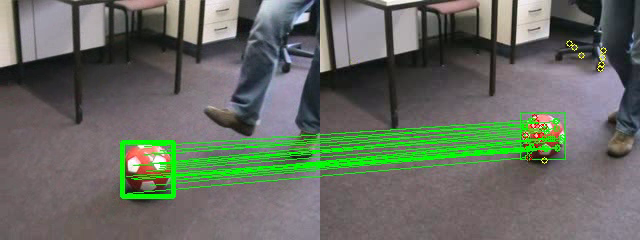
\includegraphics[width=0.95\linewidth]{imgs/matching.png}
\vspace{-2.5mm}	
\caption{Example showing how the matching precision is calculated. the image n the right shows the initial frame of the sequence. Matches in green are true positives. Circles in red are false positives. Yellow circles are false negatives, feature descriptors that are inside the object in the current frame but have a match with the background in our model.}
\label{fig:matching}
\end{figure}

Given as sequence of images $I_{1},...,I_{n}$ and the bounding box ground truth $gb_{1},...,gb_{n}$, we extract the set of target key-points descriptors $K_{1}$ from the first image of the sequence and we label all the key-points within $gb_{1}$ as descriptors of the object. For any subsequent image key-points $K_{t}$ are extracted and matched with $K_{1}$, generating a list of matches $M(i,j)_{k}$, where \textit{i} indicates a key-point descriptor of our target set $K_{1}$, and \textit{j} a descriptor of our test set. the test set is then labeled as follows:

\begin{equation}
K_{t}^{j} = 
\begin{cases}
\text{true positive}  \text{ if } K_{t}^{j} \in gb_{n} \land K_{1}^{i} \in gb_{1} \\
\text{false positive}  \text{ if } K_{t}^{j} \notin gb_{n} \land K_{1}^{i} \in gb_{1} \\
\text{false negative}  \text{ if } K_{t}^{j} \in gb_{n} \land K_{1}^{i} \notin gb_{1} \\
\end{cases}
\end{equation}

where the pair \textit{i,j} is determined by the matching result $M(i,j)_{k}$. Fig.~\ref{fig:matching} shows an example of how the key-points are labeled. The average ratio of true positives underlines the ability of a tracker to find the object and potentially recover from track loss. False negatives are feature descriptors that appear in the current frame but have no corresponding match in the initial test set $K_{1}$. This may happen due to drastic change in appearance of the object. The ratio of false positives is very important to consider since it indicates the average number of outliers that will be used to estimate the pose of the object, resulting in a bad pose estimation without employing additional filtering techniques. One widely used filtering technique consists in discarding all matched key-points if the ratio between the score of the best match and the second best match is below a certain threshold $\rho$. We define a key-point as ambiguous, if this criteria is not met. The  number of ambiguous true and false positives is then calculated to evaluate the distinctiveness of the descriptors and evaluate the influence of this common filtering technique on the results.

\subsection{Evaluating tracking precision}
\label{sec:accuracy}

\begin{algorithm}[h]
 \KwData{$I_{1},...,I_{n},b_{1}$}
 \KwResult{$b_{2},...,b_{n}$}
 $K_{1} \gets$ \textbf{extract\_points}($I_{1},b_1$)\;
 \For{$i \gets 2 : n$}{
   $K_{i}^{*} \gets$ track\_points($K_{i-1},I_{i-1},I_i$)\;
   $b_i \gets$ estimate\_pose($K_{i}^{*}$)\;
   $K_{i}' \gets$ \textbf{extract\_points}($I_{i},b_i$)\;
   $M \gets$ \textbf{match\_points}($K_{1},K_{i}'$)\;
   $K_{i} \gets$ merge\_keypoints($K_i^* ,  M$)\;
 }
 \caption{\label{alg:algorithm}Overview of the tracking algorithm used to compute the precision. The feature descriptors are employed in the steps in bold. }
\end{algorithm}

In order to measure the precision of the feature descriptors for tracking we employ a sparse key-point based tracker. The tracker requires a bounding box in the initial image of a sequence as initialization to extract feature descriptors that represent the \textit{model} of the object to track. The algorithm estimates the position of the object, represented as an oriented bounding box, with a combination of sparse optical flow and feature matching as shown in Alg.~\ref{alg:algorithm}. The original algorithm used ORB. We upgraded our algorithm making it more modular and able to cope with any possible feature descriptor. To estimate the precision we used the widely accepted overlap measure:

\begin{equation}
	\Theta (b_{t}, b_{gt}) = \frac{b_{t} \cap b_{gt}}{b_{t} \cup b_{gt}}
\end{equation}

where \textit{$b_{t}$} is the bounding box estimated by our tracker and
\textit{$b_{gt}$} is the bounding box provided by the ground truth. We define 
three precision requirements $\Upsilon$ (0.25, 0.5, 0.75) that indicates low, medium and high tracking accuracy. This is a more indicative evaluation compared to the overall accuracy. For instance, an overall value of 0.5 is ambiguous because it may indicate either a stable average accuracy around the value or a very precise evaluation in part of the video while poor in the rest.

The estimated object box \textit{$b_{t}$} is considered a true positive (TP) for a defined threshold of
accuracy $\Upsilon$ if:

\begin{equation}
\begin{cases}
b_{t} = TP  \text{ if } \Theta(b_{t}, b_{gt}) > \Upsilon \\
b_{t} = FP  \text{ otherwise }\\
\end{cases}
\end{equation}

The overall accuracy of the tracker for each precision requirement is calculated as:

\begin{equation}
\text{recall } = \frac{TP}{\text{TP } + \text{ FN}}
\end{equation}

%\missingfigure[figwidth=0.98\linewidth]{Figure showing the estimated bounding boxes and the ground truth to show the different behavior of trackers}

\subsection{Parameter setting}

All the descriptors require many parameters in order t be initialized properly. In order to evaluate the most fair comparison between them we decided to keep the values suggested by the original author of the descriptor or the implementation. However, there are some parameters that most of the feature descriptors shares that we set to the same value. The maximum number of features extracted is set to 2500 and the number of octaves is set to 4.





%% %%%%%%%%%%%%%%%%%%%%%%%%%%% CONCLUSION %%%%%%%%%%%%%%%%%%%%%%%%%%%%%%%%
\section{Conclusion}

We proposed an evaluation of the most common feature descriptors for the purpose of tracking by detection. Our experiments have shown that most of the feature descriptors have comparable results. While AKAZE and SIFT have proven to be more distinctive, ORB and BRISK compensate their weak descriptors with a higher number of points extracted. Given the growing interested in AKAZE descriptor we provided a GPU implementation so that it can be used for real time system. The code to perform the benchmark, the dataset and our implementation of AKAZE will be publicly available in order to ease researches in this area.




\bibliographystyle{unsrt}
\bibliography{ref}

\end{document}
